% !TeX program = xelatex
% !TeX encoding = UTF-8
% !TeX TXS-program:compile = txs:///xelatex | txs:///xelatex
\documentclass[aspectratio=169, table, 12pt]{beamer}

% Preamble bersama seluruh slide mata kuliah ini.
% Dipanggil dari slides/sessionXX/sessionXX.tex tepat sesudah baris
% \documentclass[aspectratio=169, table, 12pt]{beamer}
% Paket tambahan yang hanya dibutuhkan satu sesi ditulis di berkas sesi itu.

\usepackage{colortbl}
\usepackage{xcolor}
\usepackage{listings}
\usepackage{tabularx}
\usepackage{booktabs}
\usepackage{tikz}
\usepackage{pgfplots}
\usepackage{fontspec}
\usepackage[english,bahasai]{babel}
\pgfplotsset{compat=1.18}
\usetikzlibrary{arrows.meta, positioning, calc, fit, shapes.geometric,
  shapes.multipart, backgrounds, matrix, chains, trees}

\makeatletter
\def\input@path{{../theme/}}
\makeatother
\graphicspath{{../theme/}{../../figures/}}
% Stub symlink Windows memakai tema cadangan sampai aset institusi tersedia.
\IfFileExists{../theme/beamerthemePradita.sty}{%
  \usetheme{Pradita}
}{%
  \usetheme{Madrid}
  \setmainfont{TeX Gyre Heros}
  \setsansfont{TeX Gyre Heros}
  \setbeamertemplate{navigation symbols}{}
}

\definecolor{praditagreen}{RGB}{37, 113, 71}
\setbeamercolor{structure}{fg=praditagreen}
\setbeamercolor{palette primary}{bg=praditagreen,fg=white}
\setbeamercolor{palette secondary}{bg=praditagreen!80!black,fg=white}
\setbeamercolor{palette tertiary}{bg=praditagreen!60!black,fg=white}
\setbeamerfont{frametitle}{size=\large}
\setbeamertemplate{caption}[numbered]

% Ukuran header mengikuti teks agar judul panjang tidak menabrak logo.
\setbeamercolor{frametitle}{bg=white,fg=black}
\setbeamertemplate{frametitle}{%
  \begin{beamercolorbox}[wd=\paperwidth,sep=0.2cm]{frametitle}
    \begin{minipage}[c]{0.77\paperwidth}
      \raggedright\fontsize{16}{18}\selectfont\bfseries\insertframetitle
      \ifx\insertframesubtitle\empty\else
        \par\small\mdseries\insertframesubtitle
      \fi
    \end{minipage}\hfill
    \begin{minipage}[c]{0.15\paperwidth}
      \IfFileExists{../theme/classFiles/logo_universitas.png}{%
        
\includegraphics[width=\linewidth]{../theme/classFiles/logo_universitas.png}%
      }{}
    \end{minipage}
  \end{beamercolorbox}
}
\setbeamertemplate{footline}{%
  \ifnum\value{framenumber}>1
    \begin{beamercolorbox}[wd=\paperwidth,ht=0.35cm,dp=0.15cm,
      leftskip=0.3cm,rightskip=0.3cm]{palette primary}
      \footnotesize\bfseries\insertframenumber/\inserttotalframenumber
      \hfill IT40513
    \end{beamercolorbox}
  \fi
}
\DeclareRobustCommand{\berkas}[1]{\path{#1}}

% Tema membuat garis tabel berwarna putih. Dikembalikan agar tabel terbaca.
\arrayrulecolor{black}
\setlength{\arrayrulewidth}{0.5pt}

\lstdefinelanguage{yaml}{
  basicstyle=\ttfamily\scriptsize,
  keywordstyle=\color{blue}\bfseries,
  commentstyle=\color{gray}\itshape,
  stringstyle=\color{red},
  showstringspaces=false,
  breaklines=true,
  frame=lines,
  numbers=none,
  backgroundcolor=\color{lightgray!10},
  tabsize=2,
  morecomment=[l]{\#}
}

\lstdefinelanguage{json}{
  basicstyle=\ttfamily\scriptsize,
  stringstyle=\color{red},
  commentstyle=\color{gray},
  breaklines=true,
  showstringspaces=false,
  tabsize=2,
  numbers=none,
  frame=lines,
  backgroundcolor=\color{lightgray!10},
  string=[s]{"}{"}
}

\lstdefinelanguage{bash}{
  keywords={},
  basicstyle=\ttfamily\scriptsize,
  ndkeywords={docker, kubectl, helm, curl, git, terraform},
  ndkeywordstyle=\color{purple}\bfseries,
  sensitive=true,
  commentstyle=\color{gray},
  numbers=none,
  breaklines=true,
  frame=lines,
  backgroundcolor=\color{lightgray!10},
  tabsize=2,
  comment=[l]{\#},
  showstringspaces=false
}

\lstdefinelanguage{http}{
  keywords={GET, POST, PUT, PATCH, DELETE, HEAD, OPTIONS, HTTP},
  basicstyle=\ttfamily\scriptsize,
  keywordstyle=\color{blue}\bfseries,
  sensitive=true,
  numbers=none,
  breaklines=true,
  frame=lines,
  backgroundcolor=\color{lightgray!10},
  tabsize=2,
  showstringspaces=false
}

\subtitle{IT40513 · Enterprise Architecture \& Digital Blueprint}
\author{\textbf{Alfa Yohannis}}


% Sampul membatasi judul di panel putih tema rujukan Pradita.
\setbeamertemplate{title page}{%
  \begin{tikzpicture}[remember picture,overlay]
    \node[anchor=north west,inner sep=0pt,text width=8.8cm]
      at ([xshift=1cm,yshift=-3.15cm]current page.north west) {%
        {\small\insertsubtitle\par}\vspace{0.25cm}
        \resizebox{8.8cm}{!}{\begin{minipage}{12cm}
          \raggedright\color{praditagreen}\bfseries\inserttitle
        \end{minipage}}
      };
    \node[anchor=south west,inner sep=0pt]
      at ([xshift=1cm,yshift=1.65cm]current page.south west)
      {\small\insertdate};
    \node[anchor=west,inner sep=0pt,text=white]
      at ([xshift=0.8cm,yshift=0.75cm]current page.south west)
      {\small\insertauthor};
  \end{tikzpicture}
}


% Batasi kedua dimensi gambar agar diagram bersama tetap berada pada slide.
\newsavebox{\eafigbox}
\newcommand{\eadiagram}[1]{%
  \sbox{\eafigbox}{\resizebox{0.94\textwidth}{!}{\input{#1}}}%
  \ifdim\dimexpr\ht\eafigbox+\dp\eafigbox\relax>0.64\textheight
    \resizebox{!}{0.64\textheight}{\usebox{\eafigbox}}%
  \else
    \usebox{\eafigbox}%
  \fi
}


\title{\Huge Arsitektur Aplikasi\\ \vspace{10pt} dan Teknologi Saat Ini}
\date{Pertemuan 07}

\begin{document}

\begin{frame}
  \titlepage
\end{frame}

\begin{frame}
  \frametitle{Isi Pertemuan}
  \vspace{14pt}
  \begin{columns}[t]
    \column{0.5\textwidth}
    {\small\tableofcontents[sections={1-3}]}

    \column{0.5\textwidth}
    {\small\tableofcontents[sections={4-5}]}
  \end{columns}
\end{frame}

\begin{frame}{\hfill}
  \centering
  \Huge{\textbf{Bila direksi meminta daftar\\aplikasi dan biayanya, mengapa\\tiap bagian memberi\\jawaban berbeda?}}
\end{frame}

\section{Tujuan dan Konteks}

\begin{frame}{\hfill}
  \centering
  \Huge{\textbf{Tujuan dan Konteks}}
\end{frame}

\begin{frame}{{\Large Tujuan Pembelajaran}}
  \vspace{10pt}
  \begin{itemize}
    \item Menyusun katalog aplikasi dan menilainya dengan model TIME (\textit{Tolerate, Invest,
          Migrate, Eliminate}).
    \item Memetakan integrasi antaraplikasi dan menunjukkan titik rawan pola
          \textit{point-to-point}.
    \item Merangkum lanskap teknologi tingkat tinggi beserta utang teknis dan risikonya.
  \end{itemize}
\end{frame}

\begin{frame}{{\Large Masalah: Aplikasi Bertambah tanpa Rencana}}
  \vspace{10pt}
  \begin{itemize}
    \item Misalkan direktur keuangan bertanya: berapa aplikasi, berapa biaya, siapa bertanggung jawab?
    \item Bagian TI menyerahkan 19 aplikasi. Bagian keuangan menemukan 18 aplikasi lain.
    \item Para kepala unit masih menyebut 9 aplikasi yang tidak ada di kedua daftar.
    \item Tanpa potret tepercaya, modernisasi mengikuti produk yang paling terlihat.
    \item Luaran sesi ini menjadi bagian dokumen C2, ditinjau menjelang UTS.
  \end{itemize}
\end{frame}

\begin{frame}{{\Large Diagram Konsep Bab 7}}
  \centering
  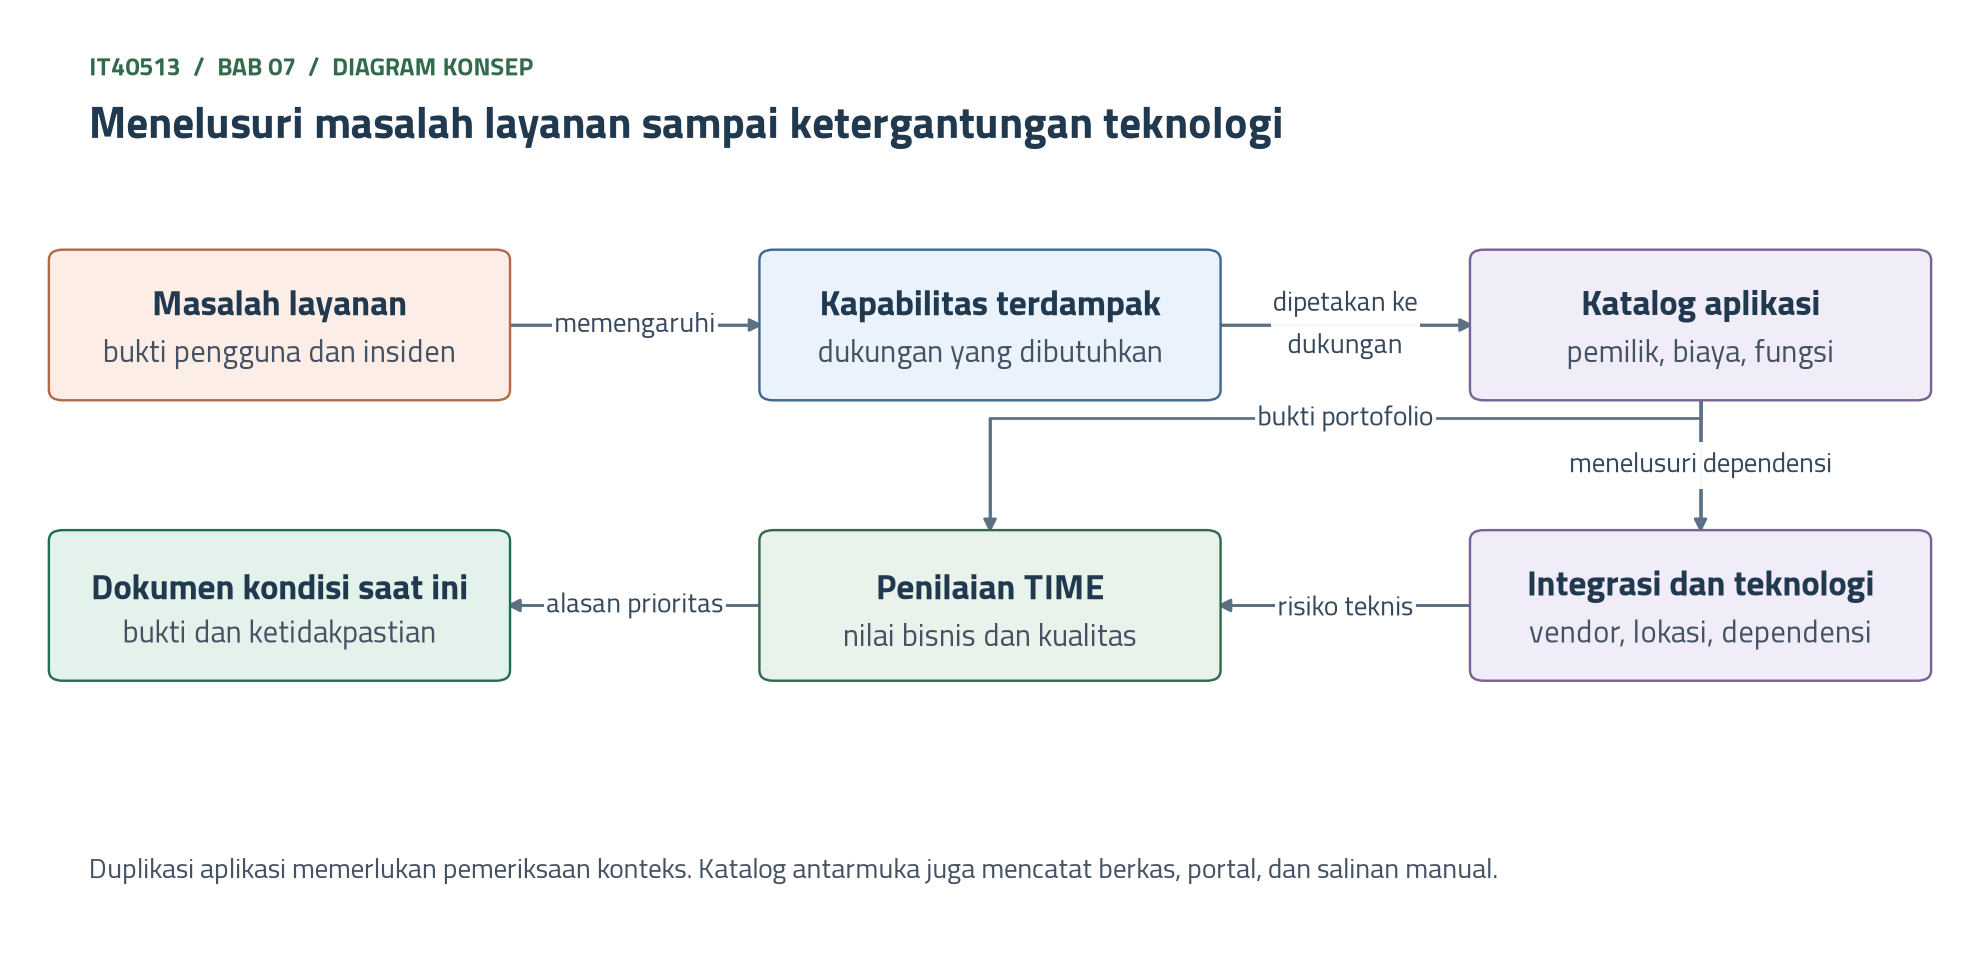
\includegraphics[width=0.96\textwidth,height=0.77\textheight,keepaspectratio]{../../figures/ch07-diagram-konsep.png}
  \label{fig:session07-ilustrasi-bab}
\end{frame}

\section{Katalog dan Penilaian Portofolio}

\begin{frame}{\hfill}
  \centering
  \Huge{\textbf{Katalog dan Penilaian\\Portofolio}}
\end{frame}

\begin{frame}{{\Large Katalog Aplikasi}}
  \vspace{10pt}
  \begin{itemize}
    \item Mencatat kode, fungsi, pemilik, pengguna, vendor, versi, umur, lokasi, dan biaya.
    \item TOGAF menyebutnya \textit{Application Portfolio Catalog}, pada fase C.
    \item Simon dan rekan: empat tahap, yaitu pengumpulan data, analisis, keputusan, optimasi.
    \item \textit{Spreadsheet} kritis tetap menjadi bagian inventaris.
  \end{itemize}
  \vspace{6pt}
  {\small Analogi: inventaris kendaraan. Merek saja tidak menunjukkan pemakai, cabang penanggung biaya,
  dan akhir perawatannya.}
\end{frame}

\begin{frame}{{\Large Rekonsiliasi Katalog Medikara}}
  \footnotesize
  \begin{tabularx}{\textwidth}{>{\raggedright\arraybackslash}p{4.3cm}cc>{\raggedright\arraybackslash}X}
    \hline
    \textbf{Sumber} & \textbf{Tambahan} & \textbf{Jumlah} & \textbf{Contoh yang ditemukan} \\
    \hline
    Katalog awal (Bab 5) & 8 & 8 & Lima SIMRS, SIM Klinik, ERP keuangan, Medikara+ \\
    \hline
    Daftar bagian TI & 11 & 19 & Sistem laboratorium, radiologi, penggajian \\
    \hline
    Kontrak pengadaan & 12 & 31 & Antrean Bandung (2021), aplikasi apotek \\
    \hline
    Tagihan unit & 6 & 37 & Langganan SaaS kecil: absensi, survei pasien \\
    \hline
    Daftar akses dan wawancara & 9 & 46 & Surveilans infeksi Bogor, Laporan Klaim Lama \\
    \hline
  \end{tabularx}

  \vspace{8pt}
  \small Angka pengandaian. Di luar 46 aplikasi masih ada 23 \textit{spreadsheet} laporan: 69 butir perlu dinilai.
\end{frame}

\begin{frame}{{\Large Unit, Pemilik, dan Jumlah}}
  \vspace{10pt}
  \begin{itemize}
    \item Unit inventaris disepakati dulu: lima SIMRS dihitung lima, SIM Klinik dihitung satu.
    \item Pemilik bisnis menjawab hasil layanan; pengelola teknis menjawab pengoperasian.
    \item Vendor mengerjakan kontrak, tidak menggantikan tanggung jawab bisnis.
    \item Mocker (273 aplikasi): hanya kerumitan saling ketergantungan yang sesuai asumsi umum.
    \item Jadi 46 aplikasi belum membuktikan pemborosan; hubungan antaraplikasi lebih penting.
  \end{itemize}
\end{frame}

\begin{frame}{{\Large Biaya Kontrak dan Biaya Penuh}}
  \footnotesize
  \begin{tabularx}{\textwidth}{>{\raggedright\arraybackslash}Xr>{\raggedright\arraybackslash}p{5.2cm}}
    \hline
    \textbf{Komponen satu instalasi SIMRS} & \textbf{Rp juta} & \textbf{Sumber bukti} \\
    \hline
    Kontrak vendor & 450 & Kontrak dan tagihan \\
    \hline
    Lisensi basis data & 280 & Kontrak lisensi \\
    \hline
    Server, sistem operasi, dan ruang server & 190 & Catatan aset dan listrik \\
    \hline
    Staf TI setempat & 220 & Alokasi waktu staf \\
    \hline
    \textbf{Biaya penuh} & \textbf{1.140} & Sekitar 2,5 kali nilai kontrak \\
    \hline
  \end{tabularx}

  \vspace{8pt}
  \small Lima SIMRS: Rp5,7 miliar, bukan Rp2,25 miliar. Tanpa pembedaan ini, kondisi saat ini tampak Rp3,45 miliar
  lebih murah.
\end{frame}

\begin{frame}{{\Large Matriks Aplikasi dan Kapabilitas}}
  \footnotesize
  \begin{tabularx}{\textwidth}{>{\raggedright\arraybackslash}Xccccc}
    \hline
    \textbf{Kapabilitas} & \textbf{SIMRS (5)} & \textbf{SIM Klinik} & \textbf{Medikara+} & \textbf{ERP} & \textbf{\textit{Spreadsheet}} \\
    \hline
    L01 Pendaftaran Pasien & U & U & P & & \\
    \hline
    L03 Penjadwalan Layanan & U & U & U & & \\
    \hline
    L04 Pengelolaan Rekam Medis & U & U & P & & \\
    \hline
    P01 Klaim dan Penjaminan & U & P & & P & P \\
    \hline
    P02 Pengelolaan Akses Pengguna & & & & & \\
    \hline
    P03 Pelaporan Manajemen & P & & & P & U \\
    \hline
    P04 Keuangan dan Akuntansi & & & & U & \\
    \hline
  \end{tabularx}

  \vspace{6pt}
  \small U: utama. P: pelengkap. $15 \times 46 = 690$ sel, dimulai dari $8 \times 4 = 32$ sel. Baris P02
  kosong: misalkan 31 dari 46 aplikasi punya akun sendiri.
\end{frame}

\begin{frame}{{\Large Model TIME}}
  \vspace{10pt}
  \begin{itemize}
    \item Dua sumbu: nilai bisnis (\textit{functional fit}) dan kualitas teknis (\textit{technical fit}).
    \item \textit{Tolerate}: menerima aplikasi apa adanya untuk sementara.
    \item \textit{Invest}: mengutamakan nilai sebesar-besarnya dari aplikasi prioritas.
    \item \textit{Migrate}: mencari aplikasi yang lebih baik untuk kebutuhan yang sama.
    \item \textit{Eliminate}: menghapus aplikasi yang tidak lagi diperlukan, setelah syaratnya terpenuhi.
  \end{itemize}
  \vspace{6pt}
  {\small Analogi: menilai bangunan cabang. Gedung penting yang rusak diperbaiki, bukan ditutup.}
\end{frame}

\begin{frame}{{\Large Kuadran TIME}}
  \centering
  \eadiagram{../../figures/ch07-time.tex}
\end{frame}

\begin{frame}{{\Large Hasil Penilaian TIME}}
  \footnotesize
  \begin{tabularx}{\textwidth}{>{\raggedright\arraybackslash}p{4.1cm}cc>{\raggedright\arraybackslash}p{1.9cm}>{\raggedright\arraybackslash}X}
    \hline
    \textbf{Aplikasi} & \textbf{Nilai} & \textbf{Teknis} & \textbf{Arah} & \textbf{Syarat} \\
    \hline
    Lima SIMRS & 5 & 1 sampai 3 & \textit{Migrate} & Layanan dan data aman \\
    \hline
    ERP keuangan & 5 & 4 & \textit{Invest} & Antarmuka tagihan diperbaiki \\
    \hline
    Medikara+ & 4 & 4 & \textit{Invest} & Akses basis data ditutup \\
    \hline
    SIM Klinik & 3 & 4 & \textit{Tolerate} & Fungsi mirip rawat jalan SIMRS \\
    \hline
    Antrean Bandung & 2 & 2 & \textit{Eliminate} & Data dua tahun dipindahkan \\
    \hline
    Surveilans infeksi Bogor & 2 & 2 & \textit{Eliminate} & Laporan dinas punya pengganti \\
    \hline
    23 \textit{spreadsheet} laporan & 2 & 1 & \textit{Eliminate} & Laporan wajib dipindah \\
    \hline
  \end{tabularx}

  \vspace{6pt}
  \small Skor pengandaian. Skala 1 sampai 5, tinggi bila 4 ke atas. Ambang adalah pilihan tim.
\end{frame}

\begin{frame}{{\Large Kasus Medikara: Sebaran 46 Aplikasi}}
  \footnotesize
  \begin{tabularx}{\textwidth}{>{\raggedright\arraybackslash}p{2.2cm}crc>{\raggedright\arraybackslash}X}
    \hline
    \textbf{Arah} & \textbf{Jumlah} & \textbf{Rp juta} & \textbf{Porsi} & \textbf{Isi utama} \\
    \hline
    \textit{Invest} & 9 & 2.900 & 23,8\% & ERP keuangan, Medikara+ \\
    \hline
    \textit{Migrate} & 11 & 6.860 & 56,2\% & Lima SIMRS (Rp5.700 juta) \\
    \hline
    \textit{Tolerate} & 14 & 1.520 & 12,5\% & SIM Klinik \\
    \hline
    \textit{Eliminate} & 12 & 920 & 7,5\% & Antrean Bandung, surveilans Bogor \\
    \hline
    \textbf{Jumlah} & \textbf{46} & \textbf{12.200} & \textbf{100\%} & \\
    \hline
  \end{tabularx}

  \vspace{8pt}
  \small Menghapus 12 aplikasi menghemat paling banyak Rp920 juta. Lima SIMRS saja menyerap 46,7 persen biaya.
\end{frame}

\begin{frame}{{\Large Dua Hal yang Sering Tertukar}}
  \vspace{10pt}
  \begin{itemize}
    \item \textit{Migrate} berbeda dari pindah ke \textit{cloud}: TIME menjelaskan arah portofolio.
    \item Pilihan teknis dianalisis bersama arsitektur target dan IT40713.
    \item TIME berbeda dari rasionalisasi: TIME menilai kondisi aplikasi saat ini.
    \item Rasionalisasi (Bab 9) memutuskan nasib aplikasi di kondisi target.
    \item Label kuadran belum menjadi rencana migrasi.
  \end{itemize}
\end{frame}

\section{Integrasi dan Antarmuka}

\begin{frame}{\hfill}
  \centering
  \Huge{\textbf{Integrasi dan Antarmuka}}
\end{frame}

\begin{frame}{{\Large Katalog Antarmuka}}
  \vspace{10pt}
  \begin{itemize}
    \item Mencatat pengirim, penerima, tujuan, data, frekuensi, pola, pemilik, dan penanganan gagal.
    \item TOGAF menyebutnya \textit{Interface Catalog}, pada fase C.
    \item Mencakup API, berkas, portal, dan langkah manual.
    \item Pertanyaan risiko: data minimum, koneksi gagal, siapa menyelesaikan selisih.
  \end{itemize}
  \vspace{6pt}
  {\small Analogi: jadwal pengiriman antarcabang. Masalahnya bukan hanya banyaknya garis, melainkan aturan tiap
  hubungan.}
\end{frame}

\begin{frame}{{\Large Empat Gaya Integrasi}}
  \footnotesize
  \begin{tabularx}{\textwidth}{>{\raggedright\arraybackslash}p{3.6cm}>{\raggedright\arraybackslash}Xc>{\raggedright\arraybackslash}p{3.8cm}}
    \hline
    \textbf{Gaya (Hohpe dan Woolf)} & \textbf{Cara kerja} & \textbf{Jumlah} & \textbf{Contoh} \\
    \hline
    Transfer berkas & Berkas dibuat lalu dibaca aplikasi lain & 11 & Klaim, tagihan \\
    \hline
    Basis data bersama & Berbagi satu basis data & 2 & Medikara+ ke Bekasi dan Bogor \\
    \hline
    Panggilan prosedur jarak jauh & Prosedur dipanggil aplikasi lain & 13 & Eligibilitas, SATUSEHAT \\
    \hline
    Pesan & Lewat sistem pesan bersama & 0 & Belum ada \\
    \hline
    \textbf{Jumlah otomatis} & & \textbf{26} & \\
    \hline
  \end{tabularx}

  \vspace{8pt}
  \small Angka pengandaian. Gaya menentukan risiko: pasangan yang sama dapat punya risiko yang jauh berbeda.
\end{frame}

\begin{frame}{{\Large Berapa Koneksi yang Mungkin dan yang Ada?}}
  \vspace{10pt}
  \begin{itemize}
    \item Sembilan sistem: lima SIMRS, ERP, Medikara+, BPJS Kesehatan, SATUSEHAT.
    \item Batas tak berarah $n(n-1)/2$: $9 \times 8 / 2 = 36$. Batas berarah: 72.
    \item Tiga mitra baru: 12 sistem, batas naik menjadi 66 pasangan.
    \item Katalog: 21 pasangan aktif, 26 antarmuka otomatis, 7 ekspor manual.
    \item Angka 36 adalah batas model, bukan jumlah antarmuka aktual.
  \end{itemize}
\end{frame}

\begin{frame}{{\Large Matriks 36 Pasangan}}
  \centering
  \eadiagram{../../figures/ch07-matriks-pasangan.tex}
\end{frame}

\begin{frame}{{\Large Integrasi Medikara Saat Ini}}
  \centering
  \eadiagram{../../figures/ch07-integrasi-saat-ini.tex}
\end{frame}

\begin{frame}{{\Large Titik Rawan Pola Point-to-Point}}
  \footnotesize
  \begin{tabularx}{\textwidth}{>{\raggedright\arraybackslash}p{4.0cm}>{\raggedright\arraybackslash}X>{\raggedright\arraybackslash}X}
    \hline
    \textbf{Titik rawan} & \textbf{Bukti} & \textbf{Akibat} \\
    \hline
    Perubahan berulang & Satu aturan klaim dikerjakan lima kali & Biaya dan peluang salah berlipat \\
    \hline
    Akses langsung ke basis data & Dua pasangan, satu akun bersama & Paparan data tidak terbatas \\
    \hline
    Keterlambatan tanpa pemantauan & SATUSEHAT rata-rata 3 hari & Kegagalan diketahui belakangan \\
    \hline
    Jalur manual & Tujuh ekspor, 144 hari-orang per tahun & Tanpa kontrol akses dan riwayat \\
    \hline
    Jalur yang tidak ada & Sepuluh pasangan antar-SIMRS kosong & Riwayat pasien tidak ikut pindah \\
    \hline
  \end{tabularx}
\end{frame}

\begin{frame}{{\Large Kasus Medikara: Biaya Integrasi per Tahun}}
  \footnotesize
  \begin{tabularx}{\textwidth}{>{\raggedright\arraybackslash}Xccccr}
    \hline
    \textbf{Kelompok} & \textbf{Pasangan} & \textbf{Antarmuka} & \textbf{Insiden} & \textbf{Perubahan} & \textbf{Rp juta} \\
    \hline
    SIMRS dan BPJS Kesehatan & 5 & 10 & 20 & 35 & 480 \\
    \hline
    SIMRS ke SATUSEHAT & 5 & 5 & 45 & 21 & 390 \\
    \hline
    Medikara+ dan SIMRS & 5 & 5 & 40 & 20 & 370 \\
    \hline
    SIMRS ke ERP & 5 & 5 & 20 & 8 & 210 \\
    \hline
    Medikara+ ke ERP & 1 & 1 & 1 & 0 & 20 \\
    \hline
    \textbf{Jumlah} & \textbf{21} & \textbf{26} & \textbf{126} & \textbf{84} & \textbf{1.470} \\
    \hline
  \end{tabularx}

  \vspace{6pt}
  \small Rata-rata Rp70 juta per pasangan aktif. BPJS Kesehatan 32,7 persen. Janji vendor 30 persen berarti Rp441 juta per tahun.
\end{frame}

\section{Teknologi dan Utang Teknis}

\begin{frame}{\hfill}
  \centering
  \Huge{\textbf{Teknologi dan Utang Teknis}}
\end{frame}

\begin{frame}{{\Large Lanskap Teknologi Medikara per Lokasi}}
  \centering
  \eadiagram{../../figures/ch07-lanskap-teknologi.tex}
\end{frame}

\begin{frame}{{\Large Dukungan Aplikasi dan Dukungan Platform}}
  \footnotesize
  \begin{tabularx}{\textwidth}{>{\raggedright\arraybackslash}p{3.9cm}cc>{\raggedright\arraybackslash}X}
    \hline
    \textbf{Produk contoh} & \textbf{Dukungan berakhir} & \textbf{Program tambahan} & \textbf{Arti bagi tim} \\
    \hline
    Windows Server 2012 R2 & Oktober 2023 & Oktober 2026 & Program pembaruan berbayar sudah habis \\
    \hline
    SQL Server 2014 & Juli 2024 & Juli 2027 & Tenggat tersisa kurang dari sembilan bulan \\
    \hline
  \end{tabularx}

  \vspace{8pt}
  \begin{itemize}
    \item Janji vendor SIMRS sampai akhir 2030 (Bab 12) belum mencakup platform di bawahnya.
    \item Standar target Bab 10: sistem operasi lama berakhir 31 Desember 2027.
    \item Tanggal diperiksa 30 Oktober 2026. Contoh publik, bukan inventaris Medikara.
  \end{itemize}
\end{frame}

\begin{frame}{{\Large Utang Teknis}}
  \vspace{10pt}
  \begin{itemize}
    \item Cunningham (1992): merilis kode pertama kali seperti berutang; bahaya muncul bila tidak dibayar.
    \item Umur bukan utang: praktisi menghargai sistem lamanya (Khadka dan rekan, 198 responden).
    \item Ramasubbu dan Kemerer: data 10 tahun, 48 perusahaan, utang menurunkan keandalan.
    \item McKinsey, 50 responden: 10 sampai 20 persen anggaran produk baru teralihkan ke utang.
    \item Angka survei adalah perkiraan sektor lain, bukan ukuran Medikara.
  \end{itemize}
  \vspace{6pt}
  {\small Analogi: pipa lama yang dirawat tidak otomatis diganti. Sambungan sementara yang menimbulkan biaya.}
\end{frame}

\begin{frame}{{\Large Pokok, Bunga, dan Keputusan}}
  \footnotesize
  \begin{tabularx}{\textwidth}{>{\raggedright\arraybackslash}p{3.7cm}>{\raggedright\arraybackslash}p{2.9cm}>{\raggedright\arraybackslash}X>{\raggedright\arraybackslash}p{3.5cm}}
    \hline
    \textbf{Utang} & \textbf{Pokok} & \textbf{Bunga} & \textbf{Keputusan} \\
    \hline
    120 modifikasi lokal SIMRS Bandung & Rp600 juta & Rp180 juta per tahun & Dibiarkan sampai SIMRS diganti \\
    \hline
    Akun bersama vendor & Rp150 juta & Peluang kebocoran berulang & Dilunasi lebih dahulu \\
    \hline
    Tujuh ekspor manual & Bergantung platform data & 144 hari-orang per tahun & Ditutup bertahap \\
    \hline
  \end{tabularx}

  \vspace{8pt}
  \small Bila SIMRS Bandung diganti dalam dua tahun, bunga yang dihindari Rp360 juta, lebih kecil daripada Rp600 juta.
\end{frame}

\section{Dokumen C2 dan Aktivitas}

\begin{frame}{\hfill}
  \centering
  \Huge{\textbf{Dokumen C2 dan Aktivitas}}
\end{frame}

\begin{frame}{{\Large Penelusuran dari Keluhan ke Teknologi}}
  \centering
  \eadiagram{../../figures/ch07-rantai-c2.tex}

  \vspace{8pt}
  \small\raggedright Pisahkan kondisi yang diamati, penilaian, dan usulan. ``Memerlukan \textit{hub}'' adalah kandidat solusi, bukan fakta.
\end{frame}

\begin{frame}{{\Large Kasus Medikara: Lima Masalah Terbesar}}
  \scriptsize
  \begin{tabularx}{\textwidth}{>{\raggedright\arraybackslash}p{3.3cm}>{\raggedright\arraybackslash}X>{\raggedright\arraybackslash}p{4.6cm}}
    \hline
    \textbf{Masalah} & \textbf{Bukti} & \textbf{Akibat} \\
    \hline
    Identitas pasien terpecah & 11,4 persen dari 10.000 nomor sampel duplikat & Riwayat klinis terpecah; tunggu obat 45 menit \\
    \hline
    Akses vendor lemah & Insiden 2025; satu akun dukungan ke API bawaan dua SIMRS & Kebocoran dapat berulang \\
    \hline
    Lima SIMRS berbeda versi & \textit{Migrate}; Rp5,7 miliar, 46,7 persen biaya & Perubahan dikerjakan lima kali \\
    \hline
    Integrasi \textit{point-to-point} & 21 pasangan, 126 insiden, Rp1.470 juta & Biaya berulang; mitra sulit ditambah \\
    \hline
    Laporan manajemen manual & 23 \textit{spreadsheet}; 144 hari-orang; selisih 2,8 persen & Terbit hari kerja ke-12 \\
    \hline
  \end{tabularx}

  \vspace{8pt}
  \small Tabel ini sengaja tidak memuat kata ``ganti'' atau ``beli''. Keputusan target menunggu Bab 8 sampai 11.
\end{frame}

\begin{frame}{{\Large Aktivitas: Peran dan Langkah}}
  \vspace{10pt}
  \begin{itemize}
    \item Analis teknologi memimpin katalog aplikasi, katalog antarmuka, dan ringkasan teknologi.
    \item Analis bisnis menilai nilai bisnis tiap aplikasi bersama penggunanya.
    \item Kedua penilaian digabung ke dalam kuadran TIME.
    \item Pemodel menggambar \textit{application cooperation view} dan \textit{technology view} di Archi.
    \item Koordinator merangkai artefak Pertemuan 4 sampai 7 dan lima masalah terbesar.
  \end{itemize}
\end{frame}

\begin{frame}{{\Large Aktivitas: Luaran dan Kriteria}}
  \vspace{10pt}
  \begin{itemize}
    \item Luaran: katalog aplikasi, diagram integrasi, ringkasan teknologi, dan dokumen C2.
    \item Kriteria, masing-masing 25 persen: inventaris, alasan penilaian, peta integrasi, konsistensi.
    \item Berkas: \berkas{sources/chapter07/README.md}.
    \item Data organisasi nyata wajib berizin dan dianonimkan.
    \item Pendalaman opsional: biaya integrasi per tahun dengan \berkas{periksa-portofolio.py}.
  \end{itemize}
\end{frame}

\begin{frame}{{\Large Ringkasan}}
  \vspace{10pt}
  \begin{itemize}
    \item Katalog: 8 aplikasi menjadi 46 setelah rekonsiliasi, ditambah 23 \textit{spreadsheet}.
    \item TIME: \textit{Eliminate} 7,5 persen biaya; lima SIMRS 46,7 persen.
    \item Integrasi: batas 36, nyata 21 pasangan, Rp1.470 juta per tahun, antar-SIMRS kosong.
    \item Teknologi: dukungan aplikasi berbeda dari dukungan platform; utang dibaca sebagai pokok dan bunga.
    \item Keputusan target memerlukan potret saat ini yang dapat ditelusuri dan dihitung.
  \end{itemize}
\end{frame}

\begin{frame}{{\Large Latihan}}
  \vspace{10pt}
  \begin{itemize}
    \item Latihan 1: aplikasi bernilai tinggi dan berkualitas teknis rendah masuk kuadran mana? Langkah apa yang wajar?
    \item Latihan 2: lima SIMRS, satu ERP, satu aplikasi pasien, dua sistem eksternal. Berapa koneksi maksimum, dan mengapa
          penting bagi direksi?
    \item Latihan 3: tiga pertanyaan untuk vendor guna menilai risiko aplikasi lama, beserta alasannya.
    \item Contoh terisi dan lembar isian ada di modul.
  \end{itemize}
\end{frame}

\begin{frame}{{\Large Bacaan dan Berkas Pendukung}}
  \small
  \begin{itemize}
    \item \href{https://aisel.aisnet.org/cais/vol26/iss1/3/}{Simon dan rekan (2010): Application Portfolio Management}
    \item \href{https://www.leanix.net/en/blog/gartner-time-tolerate}{Sheppard (2023): Gartner TIME Framework for App Rationalization}
    \item \href{https://www.enterpriseintegrationpatterns.com/patterns/messaging/IntegrationStylesIntro.html}{Hohpe dan Woolf (2003): Enterprise Integration Patterns}
    \item \href{https://doi.org/10.1287/mnsc.2015.2196}{Ramasubbu dan Kemerer (2016): Technical Debt and the Reliability of Enterprise Software Systems}
    \item \berkas{sources/chapter07/README.md}
  \end{itemize}
\end{frame}

\end{document}
